%\textbf{\large{}Unit 2, Module 4 Lab}{\large \par}
\ \\
\textbf{Name:\hrulefill{}\hspace{0.4\columnwidth}}

\textbf{Learning Goal:} For the distribution of a quantitative variable,
describe the overall pattern (shape, center, and spread) and striking
deviations from the pattern.

\textbf{Specific Learning Objectives:} Compare and contrast the distributions
of a quantitative variable for two groups using histograms. Describe
shape, give a general estimate of center and the overall range, and
calculate relevant percentages.
\begin{enumerate}
\item \textbf{Here are data from adults (247 men and 260 women) who exercise
regularly. The variable is waist girth, measured in centimeters.}\\
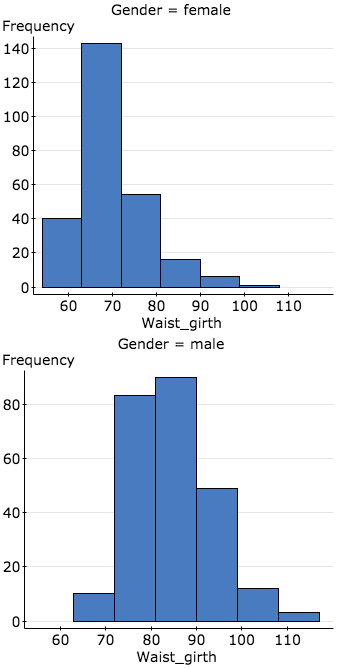
\includegraphics[width=2in]{./img/WaistGirthMF}\\
\textbf{Are the following statements valid (true) or invalid (false)?
Explain how the histograms support your answer.}

\begin{enumerate}
\item In this dataset, typical females have a smaller waist girth than typical
males.\vspace{0.5in}

\item There is less variability in waist girth for females.\vspace{0.5in}

\item Here the distributions of waist girth measurement are skewed to the
right for both males and females, with only a small percentage of
each group having waist girths exceeding 99 cm.\newpage{}
\end{enumerate}
\item \textbf{These histograms show the budget in millions of dollars for
a sample of 74 movies listed in the top 100 USA box offices sales
of all time. The movies are divided into two genres: Action/Adventure
(with 43 movies) and Other (with 31 movies).}\\
\begin{figure}[H]
\noindent \begin{centering}
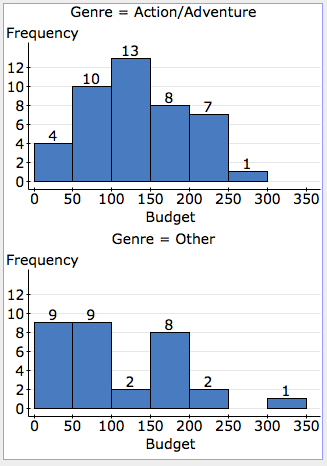
\includegraphics[clip,height=4.5in]{./img/image2}
\par\end{centering}

\end{figure}


\begin{enumerate}
\item Describe the shape of each distribution. What does the shape tell
us about where most of the data fall?\vspace{0.5in}

\item Which genre (Action/Adventure or Other) has the movie with largest
budget?\vspace{0.5in}

\item When we take all of the data into account, which genre tends to have
larger budgets? (To answer this question, give an interval that represents
typical budget amounts for each genre. Use these intervals to support
your answer.)\newpage{}
\item Which genre has more variability in budget amounts? (To answer this
question, estimate the overall range of budget amounts for each genre.
Use your estimates to support your answer.\vspace{0.7in}

\item Pick the statement that you think is more strongly supported by the
data:\\
\begin{figure}[H]
\noindent \begin{centering}
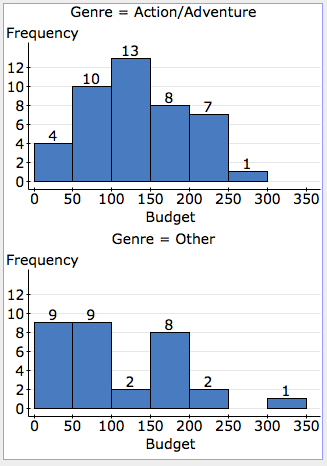
\includegraphics[height=4.5in]{./img/image2}
\par\end{centering}

\end{figure}
\end{enumerate}
\begin{itemize}
\item Action/Adventure movies tend to have larger budgets than other movies.
\item Budget amounts are similar for Action/Adventure movies and Other movies.\\
\\
For the statement you picked, support it with \emph{at least three}
precise observations from the histograms. Explain how your observations
support the statement you chose.\end{itemize}
\end{enumerate}
\clearpage


